\documentclass{tufte-handout}

\usepackage{../CommonLatexPackages/fall2018_preamble_v1.0}
\fancypagestyle{firstpage}

{\rhead{Day 3 \linebreak \textit{Version: \today}}}

\title{Welcome to Module 3: Introduction to Mobile Robotics \\
Sensory Motor Loops, Motion of Rigid Bodies }
\author{Quantitative Engineering Analysis}
\date{Spring 2019}

\begin{document}

\maketitle
\thispagestyle{firstpage}

\section{Schedule}
\begin{itemize}
\item 0900-1030: Sensory Motor Loops and Braitenberg Vehicles
\item 1030-1045: Coffee
%\item 1030-1200: Degrees of Freedom, Task Space, and Configuration Space 
\item 1045-1200: Motion of Rigid Bodies
\item 1200-1230: Overnight preview and Mathematica refresher
\end{itemize}

\section{Overview}

Welcome to Module 3!  In this module you'll be learning some of the fundamental ideas, concepts, and algorithms that lie at the heart of robotics.  Along the way we'll be revisiting some mathematical and analytical concepts we touched upon earlier in the semester.  Not only will we be applying these concepts in new contexts and to new purposes, but also extending them in important ways.  The module is structured around a series of challenges in which you will be programming your robot to perform various tasks autonomously.  As you and your robot face tougher and tougher challenges, you will need to carefully integrate a wider range of techniques in order to successfully complete the task at hand.

\section{What is a Robot?}
\begin{marginfigure}
\begin{center}
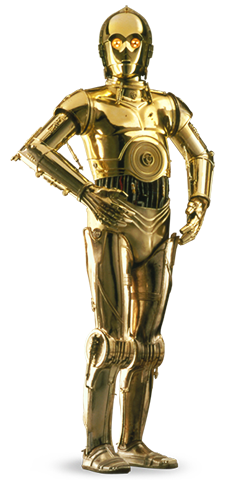
\includegraphics[width=1in]{figures/C-3PO_droid.png}
\end{center}
\caption{C-3PO from the Star Wars franchise.}
\end{marginfigure}

\begin{marginfigure}
\begin{center}
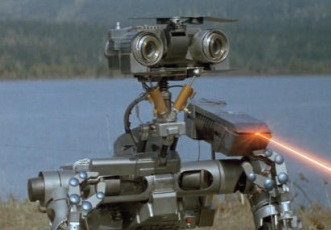
\includegraphics[width=2in]{figures/tumblr_ok5rq7U7TX1vy747uo1_500.jpg}
\end{center}
\caption{Johnny Five from the Short Circuit movies.}
\end{marginfigure}

Before diving into the challenges, let's take a step back and look at some definitions of the word ``robot''.  Merriam-Webster provides three definitions of the word.
\bi
\item a machine that looks like a human being and performs various complex acts (such as walking or talking) of a human being
\item a device that automatically performs complicated often repetitive tasks
\item a mechanism guided by automatic controls
\ei

%\begin{myboxi}[Partner Exercise]
\be[series=exercises, label=\textbf{Exercise} (\arabic*)]
\item Jot down a list of devices.  For each device, determine which, if any, of the three definitions of the word ``robot'' apply.
\ee
%\end{myboxi}


These disparate definitions highlight the fact that depending on who you ask, the answer to the question ``what is a robot?'' will likely be very different.  In a sense these three definitions proceed along a continuum of more restrictive to looser definitions, with the definition ``a mechanism guided by automatic controls'' being the loosest.  Under this definition many things that you probably wouldn't intuitively call ``robots'' are just that.  Take for example a thermostat.  A thermostat is a mechanism that automatically regulates the heat in a building by comparing the measured temperature with a ``desired'' temperature.  By the third definition, a thermostat is certainly a robot.  At this point you may be thinking that if something as simple as a thermostat is a robot, then definition 3 must be completely bogus.  After all, robots are supposed to be complicated and hard!  However, today we will see that robots can in fact be quite simple.  Further, simple robots can do some pretty complicated things.

\section{Sensory-Motor Loops}

\begin{marginfigure}
\begin{center}
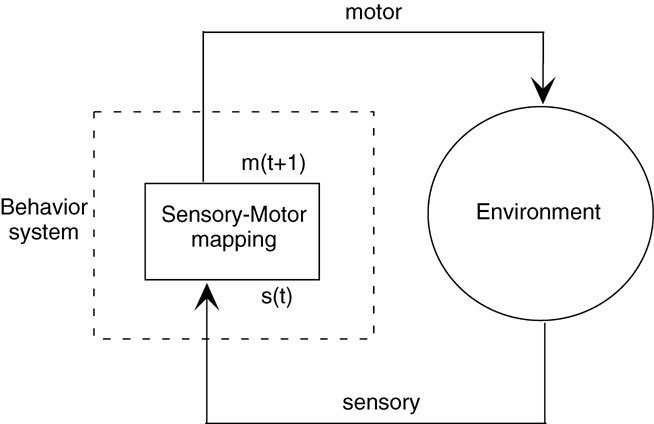
\includegraphics[width=2in]{Figures/fnbot-01-002-g001.jpg}
\end{center}
\caption{A schematic of a robot controlled by a sensory-motor loop.\label{fig:sensorymotorloop}}
\end{marginfigure}

We ended our last section on a somewhat cryptic note.  If we seek to design simple robots, how on earth can they do complex things?  The answer to this question lies in the fact that robots are not isolated machines, but instead interact with a complex and ever-changing world.  A simple model that captures this idea is the sensory-motor loop (see Figure~\ref{fig:sensorymotorloop}).  The model situates the robot within an environment that it interacts with through two pathways.

The first is a \textbf{motor pathway} by which the robot executes actions which affect its environment.  In our thermostat example these actions would be turning the heating system on or off.  In a more conventional example of a robotic arm in a manufacturing plant, this could be operating the motors that control the joints of the arm.

The second is a \textbf{sensory pathway} by which the robot perceives its environment.  In our thermostat example this could be a temperature sensor such as a thermocouple.  In the case of a robotic arm in a manufacturing plant, this could be a potentiometer that measures the angle of each of the arm's joints or pressure sensors that measure contacts between the robot arm and other objects.

The ''brain'' of the robot, if you will, is defined by the box labeled ``behavior system''.  In the general case you could imagine that the robot's brain might integrate multiple pieces of sensory information over time to form representations of the world around it. Take for example a robot mapping a building. The robot could build a progressively more detailed map by moving around in the building and collecting sonar readings (which provide an estimate of distance to objects in the world) over time.  Putting aside this more complex form, let's restrict ourselves to robots with fairly simple behavior systems. \textbf{What about a robot that has no memory at all?} Such a robot would have to make all of its decisions based on its current sensory information.

%\vspace{1em}
%\begin{myboxi}[Partner Exercise]
\be[resume=exercises, label=\textbf{Exercise} (\arabic*)]
\item Design robots using the model in Figure~\ref{fig:sensorymotorloop}.  Restrict yourselves to robots that have no memory (i.e. ones that act at any moment in time directly based on their sensory input).  To help get your creative juices flowing, it may help to make lists of sensors and actuators.  You can then create interesting ideas by seeing what would happen if you paired a particular sensor with a particular actuator in a particular context.  Don't worry too much about trying to design useful robots (whimsical is good), the goal here is to be creative and to think through the mental simulations necessary to understand how your robot would behave.  Here are some suggestions for sensors and actuators.

\textbf{Sensors:} vibration sensor, microphone, camera, thermal camera, wheel rotation sensor, pressure sensor, light intensity sensor, laser range sensor, bump detector, temperature sensor, breathalyzer, etc.  (Wikipedia has \href{https://en.wikipedia.org/wiki/List_of_sensors}{a good list}).

\textbf{Actuators:} DC motors, combustion engines, stepper motors, solenoids, speakers, laser beams, LEDs, etc.
%\end{myboxi}
\ee

\section{Grey Walter's Tortoises}
\begin{marginfigure}
\begin{center}
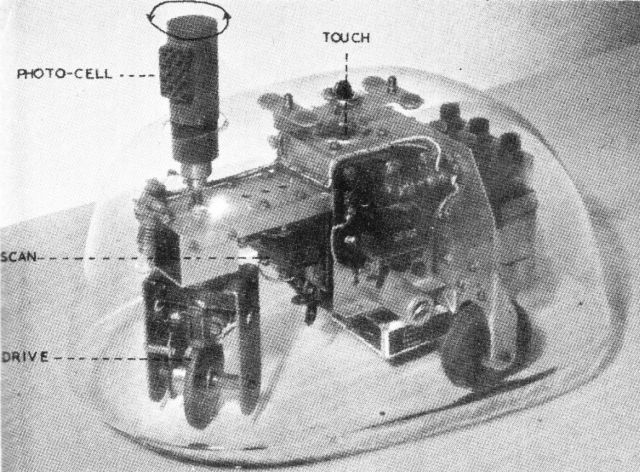
\includegraphics[width=2in]{Figures/WGW-Discussions-x-pics-x640.jpg}
\end{center}
\caption{Gray Walter's Tortoise Elsie\label{fig:tortoise}}
\end{marginfigure}
Two very early examples of electric robots that worked using the principle of sensory-motor mappings were Grey Walter's robotic ``Tortoises'' Elmer and Elsie (see Figure~\ref{fig:tortoise}).  This \href{https://www.youtube.com/watch?v=lLULRlmXkKo}{YouTube video} probably tells the story better than we possibly could.

As Grey Walter said himself, the robots behave as if they had a very simple two-cell nervous system that specifies the sensory-motor mapping (or behavior system).  Despite this striking simplicity, the robots are capable of complex behavior such as obstacle avoidance and phototaxis (navigating towards the light that marks the charging kennel).  This is an example of what we've been alluding to several times in this document: simple sensory-motor mappings can lead to complex behavior when put into a complex environment.

\section{Braitenberg Vehicles}
The pioneering work of Grey Walter was followed up by a number of others.  One particularly interesting work was by Valentino Braitenberg. Valentino Braitenberg was interested in how vehicles controlled by very simple sensory-motor loops could execute behaviors that when viewed by humans would cause them to ascribe emotion and feelings of intelligence and intentionality to these vehicles. The name typically used to refer to these hypothetical robots is ``Braitenberg Vehicles''.  While Braitenberg never actually built these vehicles (he was more interested in how these simple vehicles might inform various philosophical issues, particularly in the area of philosophy of mind), others have followed up and actually built these vehicles.  \href{https://www.youtube.com/watch?v=VWeRC6j0fW4}{Here is a video} from a group at MIT that built several of Braitenberg's vehicles.

\begin{marginfigure}
\begin{center}
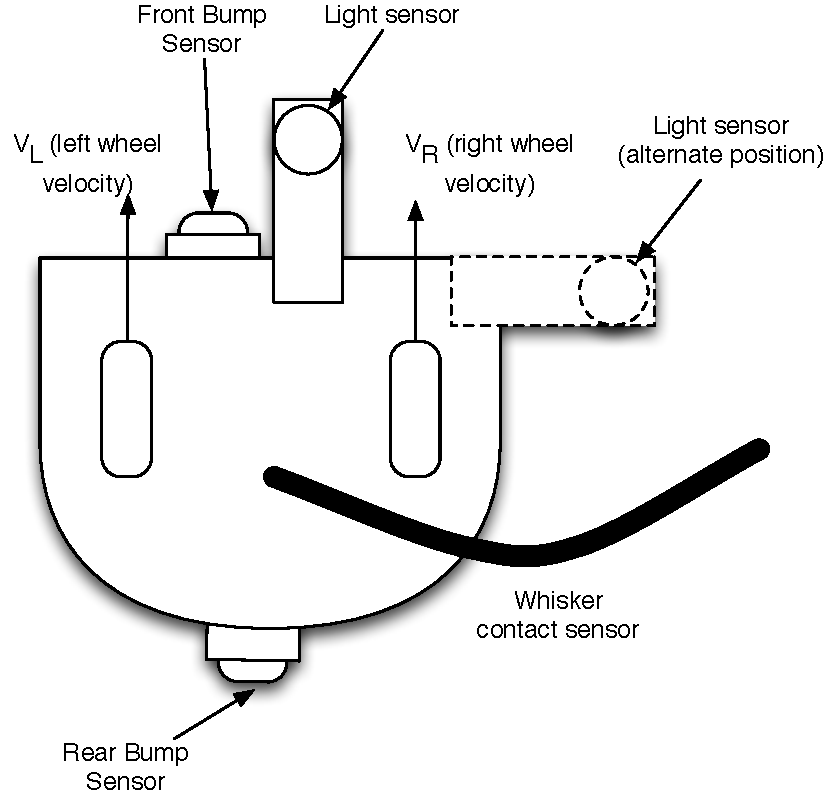
\includegraphics[width=2in]{Figures/robotschematic}
\end{center}
\caption{A schematic of the vehicle from the \href{https://www.youtube.com/watch?v=VWeRC6j0fW4}{real-life Braitenberg vehicles video}.  The robot is a differential drive vehicle with two wheels.  We use $V_L$ and $V_R$ to refer to the velocities of the left and right wheels (positive is forward by convention).  Also labeled are the other sensors on the robot, including the light sensor that reads higher values when exposed to more light, a whisker sensor that reads 0 when it is not in contact with something and 1 if it is, and two bump sensors that read 1 when they hit something and 0 otherwise.\label{fig:braitenbergschematic}}
\end{marginfigure}

A schematic of the vehicle (or robot) in the video is shown in Figure~\ref{fig:braitenbergschematic}.  The robot has two motors that each control one of the robot's wheels.  We can use the symbols $V_L$ and $V_R$ to refer to the velocities of each of the wheels (positive indicating a forward velocity).  Using the framework from the previous section, these are our actuators.  The robot also has a number of sensors.  A light sensor outputs a continuous value which reads out larger values when in the presence of bright light and smaller values in the presence of low light (this is basically a one-pixel camera!).  Additionally the robot has two bump sensors that have binary outputs.  That is, they output 1 when they strike an object and 0 otherwise.  Finally, the robot has a whisker sensor that is also binary and outputs a 1 when it contacts something and 0 otherwise.

Before getting on to the task of figuring out how one might program a robot like this, we need to understand a bit about how the drive systems of these robots work.  The configuration shown in Figure~\ref{fig:braitenbergschematic} is known as \emph{differential drive}.  We will be thinking much more systematically about differential drive in the first robot challenge, but for now let's try to understand it from a qualitative perspective.

%\begin{myboxi}[Partner Exercise]
\be[resume=exercises, label=\textbf{Exercise} (\arabic*)]
\item To build a qualitative understanding of differential drive it helps to understand a few limiting cases.  Good ones to start with are ones that involve the wheels moving at equal speeds in either the forward (positive) or reverse (negative) direction.  In these cases the robot will either move forward in a straight line or backwards in a straight line.  In these cases the speed of the robot is directly proportional to the speed of its wheels.  Now, let's consider cases where the velocities of the two wheels are unequal.  To help you with your intuition it might help to imagine the right wheel pulling either forwards or backwards on the right side of the robot and the left wheel pulling either forwards or backwards on the left side of the robot.  Here is a potential list of limiting cases to consider.  Make predictions about what would happen in these cases.  It may help to sketch a couple of key frames (poses of the robot) over time.
\be
\item What if $V_L$ is positive and $V_R = -V_L$?
\item What if $V_R$ is positive and $V_L = -V_R$?
\item What if $V_L = 0$ and $V_R$ is positive?
\item What if $V_R = 0$ and $V_L$ is positive?
\item What if $V_L = 0$ and $V_R$ is negative?
\item What if $V_R = 0$ and $V_L$ is negative?
\item What if $V_R$ is positive and $V_L = \frac{1}{2}V_R$?
\item What if $V_L$ is positive and $V_R = \frac{1}{2}V_L$?
\ee
\ee

\section{Programming a Robot on a Whiteboard}
Next, you will be programming this vehicle to perform the behaviors you saw in the video.  However, instead of programming the robot using a computer, you will be programming it at the whiteboard.  How can you program using a whiteboard (we imagine you conveniently might ask)?!?  Remember, we are thinking of our robot's brain as a sensory-motor mapping.  Translated into the language of mathematics this simply means that our robot program is specified by a function from sensors to motors!

There are many ways to represent a function.  One way is as an equation.  For instance, a robot that moves faster and faster as it see more and more light could have $V_L(\ell) = \ell^2$ and $V_R(\ell) = \ell^2$ (where $\ell$ is the intensity of the light measured by the light sensor).  Another way to represent a function is to define it graphically.  You could draw a function that has $\ell$ on the x-axis and $V_L$ on the y-axis.  You could then sketch the relationship between those two quantities.  Doing this graphically you could either have a quantitatively accurate sketch or a sketch that simply characterizes the qualitative behavior of the function.  For sensors that have binary values, like the bump sensors, you can exhaustively enumerate all conditions.  For instance, here is the program of a robot that drives forward at a $0.5 \frac{m}{s}$ until it rams into something
\begin{align}
V_L(bump_F) = \begin{cases} 0.5 \frac{m}{s},  ~~bump_F = 0   \\ 0\frac{m}{s}, ~~~~bump_F = 1\end{cases} \nonumber \\
V_R(bump_F) = \begin{cases} 0.5 \frac{m}{s},  ~~bump_F = 0 \\ 0\frac{m}{s}, ~~~~bump_F  = 1\end{cases} \nonumber
\end{align}
where $bump_F$ is the value of the forward bump sensor (1 when in contact with something, 0 otherwise).

%\vspace{1em}
%\begin{myboxi}[Partner Exercise]
\be[resume=exercises, label=\textbf{Exercise} (\arabic*)]
\item Work through generating robot programs to realize the behaviors in the video.  Questions and considerations to keep in mind while doing this activity are:
\be
\item In order to validate your proposed program, it helps to do a quick whiteboard simulation.  Sketch out a few key instants in time, what the robot's sensors would read, and what the wheel velocities would be.
\item At least one of the behaviors cannot be reproduced without some primitive form of memory (although perhaps if you are very creative it can work).  Which behaviors are these?  How can you tell?
\ee
\ee

Next, Imagine your robot can remember a small amount of information.   Specifically, your robot has access to a single flag that starts out with the value 0.  Its value can be toggled from 0 to 1 or from 1 to 0 when a particular event occurs.  For instance, if the light sensor reads a certain value, the robot might toggle its flag.  The value of the flag can then inform the behavior of the robot. Given this new capability, implement any behaviors in the video that you couldn't before.

%\vspace{1em}
If you get done earlier than other groups, consider adding an additional light sensor to your robot.  Now that you have two light sensors, you can get the robot to do a richer set of behaviors.  Sketch the configuration of sensors on your new Braitenberg vehicle (equipped with two light sensors).  Try to reproduce behaviors such as light seeking and light avoiding.  For more ideas see \href{https://en.wikipedia.org/wiki/Braitenberg_vehicle}{the Wikipedia page on Braitenberg vehicles}.

%\end{myboxi}

\section{Coffee [15 minutes]}

%\section{Degrees of Freedom and Configuration Space [1 hour 40 minutes]}
%
%\begin{marginfigure}
%\begin{center}
%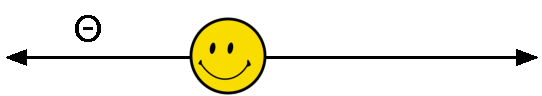
\includegraphics[width=2in]{Figures/liney}
%\caption{Liney the very happy 1-dimensional robot.\label{fig:liney}}
%\end{center}
%\end{marginfigure}
%We started off class by examining robots that move through space by adjusting the velocities of their wheels.  Next, we will learn some general terminology to frame robot motion of all different types.  To get us started, let's consider a very simple robot.  This robot, let's called it ``Liney'', can move itself forwards and backwards along a line (see Figure~\ref{fig:liney}).  Let's call the robot's position along the line $\theta$.  In this case $\theta$ is known as the \emph{configuration space} of the robot Liney.  The \emph{configuration space} of a system is the set of generalized coordinates which are necessary to completely define the positional configuration of the system.  In this case, $\theta$ is a full and complete specification of the configuration of our robot.
%
%\begin{marginfigure}
%\begin{center}
%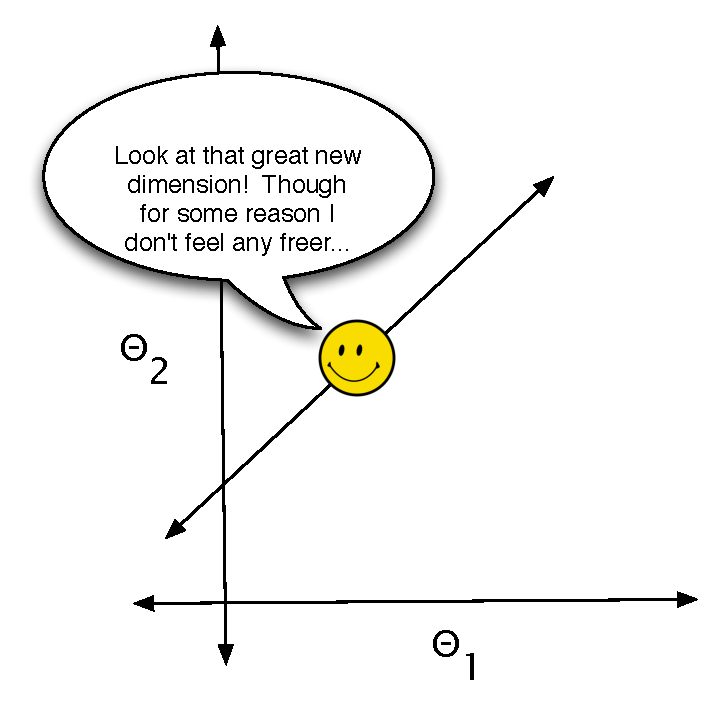
\includegraphics[width=2in]{Figures/liney_in_plane}
%\caption{Liney the very happy 1-dimensional robot has now moved to a planar world!\label{fig:liney_in_plane}}
%\end{center}
%\end{marginfigure}
%One important property of the configuration space is the number of \emph{degrees of freedom}. The \emph{degree of freedom} of a system is the number of independent quantities which must be specified to fully determine the configuration of the system.  This clearly depends on the number  of coordinates in the configuration space, but also on what the constraints are that exist in the space (i.e. particular configurations that cannot physically be realized).  For Liney, we can say that it has 1 degree of freedom.  We didn't really specify enough information to say whether or not there are any constraints on its position, so we'll assume that there are none.  Now, however, let's move Liney's line to live in a plane (see Figure~\ref{fig:liney_in_plane}).  Now we need two coordinates to fully define Liney's position, however, the constraint that Liney needs to always be on the line reduces the number of degrees of freedom to 1.
%
%As a second example, consider a planar, two-link robot arm, which unfortunately doesn't have a cute or humorous name (see Figure~\ref{fig:2darm}).  The two joint angles, $\theta_1$ and $\theta_2$, define the configuration space of this robot.  Further, let's assume that the joint angles are each independently controllable via servo motors.  Since the dimensionality of our configuration space is 2 (i.e. there are 2 joint angles that define the configuration of our robot), and each joint can move independently we say that this robot has 2 degrees of freedom.  Depending on the range of motion of each of our joints, we may also say that our configuration space has some constraints.  For instance, perhaps $0 \leq \theta_1 \leq \pi$ and $0 \leq \theta_2 \leq \pi$ --- indicating that the joints have a 180 degree maximum range of motion.  These constraints do not limit the number of degrees of freedom of the system, however.
%\begin{marginfigure}
%\begin{center}
%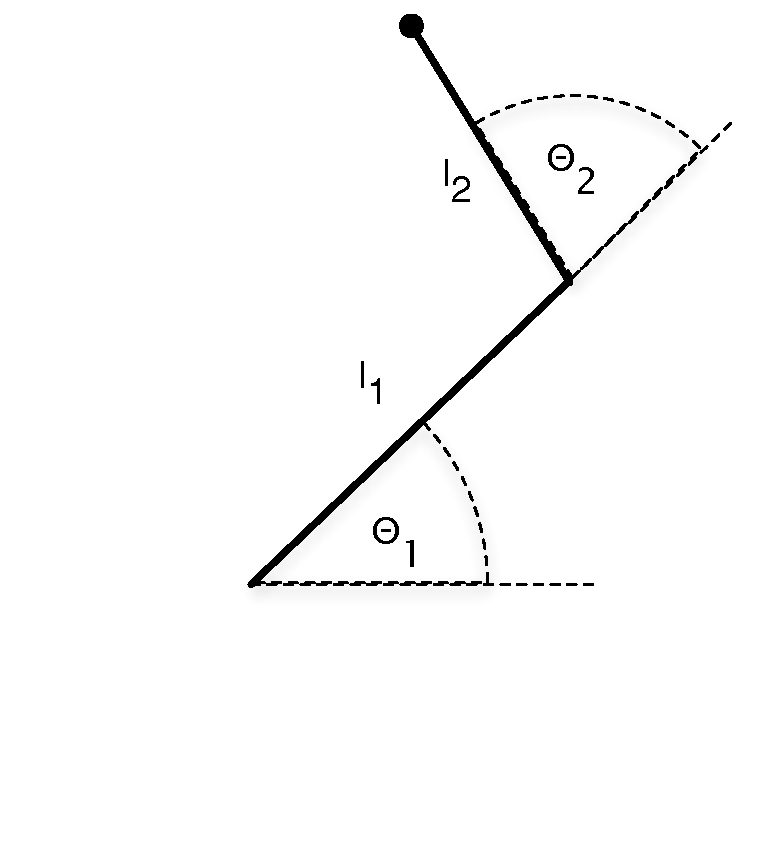
\includegraphics[width=2in]{Figures/2darm}
%\caption{A schematic of a 2D planar arm.  The joint angles are given by $\Theta_1$ and $\Theta_2$.  The lengths of the two links are given by $l_1$ and $l_2$.\label{fig:2darm}}
%\end{center}
%\end{marginfigure}
%
%As a final example consider a tricycle (see Figure~\ref{fig:tricycle}).  We can define the configuration of the tricycle with four dimensions, $\theta_1$ is the steering angle of the tricycle's front wheel, $\theta_2$ is the tricycle's x-position in the world, $\theta_3$ is the tricycle's y-position in the world, and $\theta_4$ is the tricycle's heading (rotational position of the body of the tricycle).  Since there are no constraints between the dimensions of the configuration space, this system has 4 degrees of freedom.  In contrast to our previous examples, if we are riding the tricycle, only $\theta_1$ is directly controllable.  Of course we can also control the velocity of the front wheel, however, that is not part of the configuration space. The reason for this is, as we discussed earlier, the configuration space only specifies \emph{positional} components of the configuration. The other dimensions of the configuration space (e.g., x-position, y-position) can be influenced by manipulating $\theta_1$ and the front wheel velocity over time.
%
%\begin{marginfigure}
%\begin{center}
%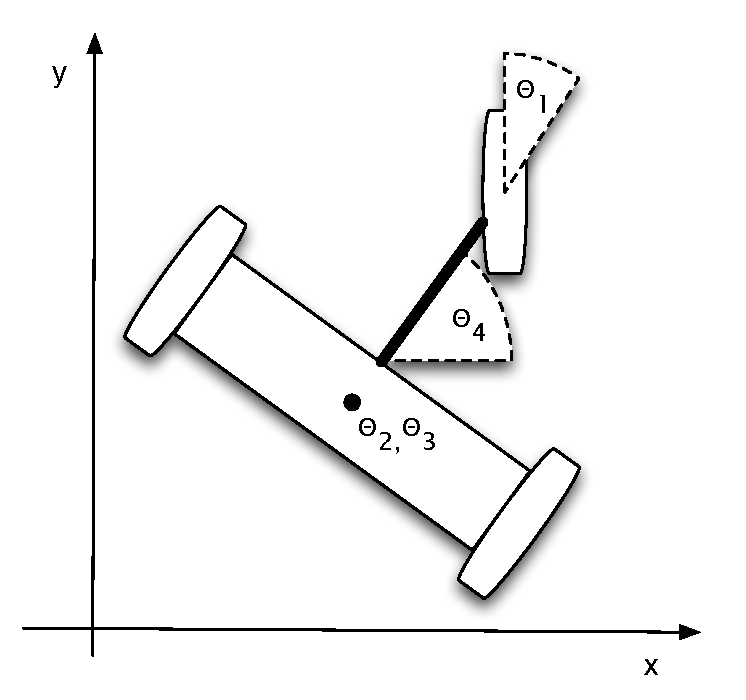
\includegraphics[width=2in]{Figures/tricycle}
%\caption{A schematic of a tricycle.\label{fig:tricycle}}
%\end{center}
%\end{marginfigure}
%
%\vspace{1em}
%\begin{myboxi}[Partner Exercise]
%For each of the systems below, define the configuration space by drawing a diagram of the system and labeling each coordinate.  Determine whether there are any constraints on the configuration space and what the degree of freedom of the system is.  Many of these questions have more than one reasonable answer, so focus on your chain of reasoning rather than arriving at uniquely correct answers.
%\begin{enumerate}
%\item A point translating in $\mathbb{R}^2$ (two dimensional space:  a plane)
%\item A bar translating and rotating in $\mathbb{R}^2$
%\item A point translating in $\mathbb{R}^3$ (three dimensional space: like our world)
%\item A 2D vector expressed in polar coordinates with $r$ constrained to be 1.
%\item A vector in $\mathbb{R}^3$ with unit length.
%\item A 256 by 256 pixel image of a face reconstructed as a linear combination of $40$ Eigenfaces.
%\item A 3D, unit vector whose direction is given by a horizontal angle and a vertical angle.
%\item A human arm
%\item A car
%\item A bike
%\item A rollercoaster
%\item A planar robot arm with three joints
%\end{enumerate}
%\end{myboxi}
%
%\section{Task space}
%
%Many times we don't care about the configuration of our robot directly, but instead want our robot to reach some position in the world.  Take for example a robot on a factory assembly line.  In order to tighten a screw on a product being assembled, the robot's end-effector (or gripper) must move to the correct position in space.  In the case of a wheeled robot we may be interested in guiding it to some goal position (e.g., to complete a delivery).  The space in which the robot performs its task is known as \emph{task space}.  Revisiting the two examples just presented, the task space of the robot arm is the position of the end-effector of the robot arm.  For the wheeled delivery robot, the task space is the x-y position of the robot.
%
%\vspace{1em}
%\begin{myboxi}[Partner Exercise]
%For each of the following robots,
%\begin{enumerate}
%\item A planar robot arm with two joints that seeks to grab an object with its end-effector.  The configuration space consists of the two joints of the robot.
%\item A planar robot arm with three joints that seeks to grab an object with its end-effector.  The configuration space consists of the three joints of the robot.
%\item Liney the robot in its new 2-dimensional home (see Figure~\ref{fig:liney_in_plane}).  For this problem consider the configuration space to be its position along the line to which it is constrained (note: this is in contrast to the configuration space shown in the figure).  Since Liney's purpose in life is not clear, let's just assume its task space is its $x,y$ position in the world.
%\end{enumerate}
%
%do the following exercises.
%\begin{enumerate}[label=(\alph*)]
%\item Define the robot's task space by drawing a diagram that shows both the task space and configuration space of the robot.
%\item Determine any constraints on the points in the task space that are achievable.  Your answer to this need not be in the form of an equation, for instance, you could describe the constraints in words.
%\end{enumerate}
%\end{myboxi}
%
%\section{Forward Kinematics}
%The mapping from configuration space to task space is known as the forward kinematics of a robot.  Solving the kinematics problem is one of the first steps to being able to control a robot.  In the challenge for this week we'll be solving this problem for a differential drive robot.  In class today, we'll address the problem of solving the kinematics of a robotic manipulator (see the \href{https://en.wikipedia.org/wiki/Serial_manipulator}{Wikipedia page on serial manipulators} for more information on these mechanisms).  Recall that for a robotic manipulator, the task space is the $x, y$ position of the end-effector (or gripper) of the manipulator.  Thus, the forward kinematics problem is to map from the joint angles of the manipulator (or configuration space) to this $x,y$ position.
%
%\vspace{1em}
%\begin{myboxi}[Partner Exercise]
%\begin{enumerate}[label=(\alph*)]
%\item Determine the forward kinematic equations for the robot arm shown in Figure~\ref{fig:2darm}.
%\item Do the same for a 3-link, planar robot arm.  You are free to design the geometry of this arm yourself.
%\item Do the same for a 3-link, planar robot arm that has a linear joint instead of a rotational joint between the its second and third link.  A linear joint is one where the motion is linear instead of rotational.
%\end{enumerate}
%\end{myboxi}
%
%\section{Inverse Kinematics}
%The mapping from task space to the configuration space is known as the inverse kinematics problem.  In the challenge for this week we'll be determining the inverse kinematics of a differential drive robot.  Before we begin, let's crisply state what it is we are trying to do.  We are trying to compute the the joint angles necessary to place the robot's end effector at a particular $x, y$ position.  The procedure for determining the equations that relate $x$ and $y$ to the joint angles of the robot is somewhat intricate, however, it only uses basic concepts from trigonometry (e.g., law of cosines, arc tangents).  For a good step-by-step derivation, check out Example 4.2 of \href{https://ocw.mit.edu/courses/mechanical-engineering/2-12-introduction-to-robotics-fall-2005/lecture-notes/chapter4.pdf}{MIT's Open Courseware Writeup} of the topic.
%
%\vspace{1em}
%\begin{myboxi}[Partner Exercise]
%Without doing any calculations, determine whether or not the inverse kinematics problem has a unique solution for a three-link planar robotic manipulator.  How about for a two-link planar robotic manipulator?  Draw pictures to justify your answers.
%\end{myboxi}

\section{The Motion of Rigid Bodies [75 mins]}

We are going to explore the concept of angular velocity using an "app" for your phone. Please download and install "SensorKinetics" to your phone, and open the "Gyroscope sensor". 
%\begin{myboxi}[Partner Exercise - Qualitative]
\be[resume=exercises, label=\textbf{Exercise} (\arabic*)]
\item {\bf Qualitative}: For each of the questions below, you should "plot" the data on the board, and interpret the data qualitatively in terms of the coordinate system of the phone.
\be
\item Place your phone on the table and spin it, in place, counterclockwise. Note that you should be spinning it about an axis that is orthogonal to the face of the phone. Which axis is this on the data graph? What happens if you spin it clockwise?
\item Now spin the phone about the two other axes. Which axis is which? Which direction is clockwise and which is counterclockwise? Clearly draw the coordinate system the phone is using - use the unit vectors $\hat{\x}$, $\hat{\y}$, and $\hat{\z}$. 
\item What happens if you move the phone along a straight line (on the table) without turning the phone?
\item What happens if you move the phone uniformly in a circle {\bf without turning the phone}? i.e. the orientation of the phone does not change.
\item What happens if you move the phone uniformly in a circle {\bf while turning the phone at the same time}? i.e. imagine the phone is a car and you are driving in a circle.
\ee
\ee
%\end{myboxi}

Now that we've explored angular velocity using the phone, let's make it quantitative. We will use the following notation for the angular velocity
\[ \boldsymbol \omega = \omega_x \hat{\x} + \omega_y \hat{\y} + \omega_z \hat{\z} \]
so that $\omega_x$ is the component of angular velocity corresponding to rotation about the x-axis and so on. The units of angular velocity are in radians per second, e.g., rotating in a complete circle in one second would be a $2 \pi$ radian/second rotation.

%\begin{myboxi}[Partner Exercise - Quantitative]
\be[resume=exercises, label=\textbf{Exercise} (\arabic*)]
\item {\bf Quantitative}: For each of the questions below, you should "plot" the data on the board, and interpret the data quantitatively in terms of the coordinate system of the phone.
\be
\item Predict the angular velocity if you place the phone down on the table and then spin the phone in place so that it spins once in 5 seconds. Confirm your prediction using the data.
\item Predict the angular velocity if you uniformly move the phone in a circle in 5 seconds, and confirm your prediction using the data. Does it matter how large the circle is?
\item What type of motion would give rise to a constant $\omega_z$ of 2 radians per second for 5 seconds, with both $\omega_x = 0$ and $\omega_y = 0$? Confirm your prediction with the phone.
\item What type of motion would give rise to a sinusoidal $\omega_z$ with amplitude of 2 radians per second, and a period of 10 seconds, with both $\omega_x=0$ and $\omega_y=0$.
\item What type of motion would give rise to a constant $\omega_z$ and $\omega_x$ of 2 radians per second for 5 seconds, with $\omega_y=0$. Confirm your prediction with your phone.
\item Sketch a graph of your own choosing of $\omega_x$, $\omega_y$, and $\omega_z$ and challenge yourself to produce it using the phone!
\ee
\ee
%\end{myboxi}

Hopefully we have a qualitative and quantitative sense for angular velocity now.  The angular velocity is a vector with magnitude and direction. We've seen that the direction is the axis of rotation (and counterclockwise is positive), and the magnitude is defined as the rate of change of the angle in rad/s. For example, if we use $\theta_x$ to represent the angle of rotation about the x-axis, then the x-component of the angular velocity is
\[ \omega_x = \frac{d \theta_x}{dt} \]
Although the literature tends to use different Greek letters to represent the different angles of rotation in 3D, we will use $\theta_x$, $\theta_y$, and $\theta_z$ for simplicity.

Since the angular velocity is the time derivative of the angle, the angle must therefore be determined by the integral of the angular velocity
\[ \theta_x(t) = \theta_x(0) + \int_0^t \omega_x(t) \; dt \]
where $\theta_x(0)$ is the initial angle at $t=0$. In the case where the angular velocity is constant the integral gives
\[ \theta_x(t) = \theta_x(0) + \omega_x t \]
which means that the angle increases linearity in time as expected - that rate of increase is just the angular velocity. {\bf If the angular velocity is not constant, we need to integrate it in time to determine the angle.}

%\begin{myboxi}[Partner Exercise - Mathematical]
\be[resume=exercises, label=\textbf{Exercise} (\arabic*)]
\item {\bf Mathematical:} For each of the following questions you should carry out the relevant integral, and think about the motion of the phone.
\be
\item Determine $\theta_z(t)$ if $\omega_z(t) = 2$ radians per second. Describe the motion of the phone in this case.
\item Determine $\theta_z(t)$ if $\omega_z(t) = \alpha t$ radians per second. Describe the motion of the phone in this case.
\item Determine $\theta_z(t)$ if $\omega_z(t) = \sin(\alpha t)$ radians per second. Describe the motion of the phone in this case.
\ee
\ee
%\end{myboxi}

We will finish this exploration by connecting back to rotation matrices from earlier in this module. We will now use MATLAB to define a set of unit vectors corresponding to the coordinate system of the phone, and we will use rotation matrices to rotate these unit vectors.

%\begin{myboxi}[Partner Exercise - Computational]
\be[resume=exercises, label=\textbf{Exercise} (\arabic*)]
\item Look up and write down the rotation matrices for 3D rotations - use $\theta_x$, $\theta_y$, and $\theta_z$ for the angles.
\item In MATLAB, define a set of unit vectors $\hat{\x}$, $\hat{\y}$, and $\hat{\z}$ in 3D. For example,
\begin{verbatim}
>> xhat = [1;0;0]
\end{verbatim}
Use "quiver3" to plot these unit vectors in 3D with the origin at $(0,0,0)$. Now choose a specific rotation angle about each of the axes in turn, transform the vectors by multiplying with the rotation matrix, and use "quiver3" to visualize the new vectors to confirm the rotation matrix does what you expected.
\item Now write a "for" loop that rotates the unit vectors in 3D for the following scenarios so that you can produce an animation - you will need to issue the "drawnow" command so that the graphic updates every time you issue the quiver3 command. 
\be
\item $\omega_z = 2$ radians per second, and $\omega_x=\omega_y=0$.
\item $\omega_x = 2$ radians per second, and $\omega_y=\omega_z=0$.
\item $\omega_y = 2$ radians per second, and $\omega_x=\omega_z=0$.
\item $\omega_z = \omega_x = 2$ radians per second, and $\omega_y=0$.
\item $\omega_z = 2t$ radians per second, and $\omega_x=\omega_y=0$.
\item $\omega_z = \sin(2 t)$ radians per second, and $\omega_x=\omega_y=0$. 
\ee
\item {\bf Challenge (if you have time)} Record some data with the phone, upload it to MATLAB, and try to produce an animation of the unit vectors identical to the motion of the phone. 
\ee
%\end{myboxi}


\section{Overnight preview and Mathematica refresher [30 mins]}

\end{document}
